%%%%%%%%%%%%%%%%%%%%%%%%%%%%%%%%%%%%%%%%%
% University/School Laboratory Report
% LaTeX Template
% Version 3.1 (25/3/14)
%
% This template has been downloaded from:
% http://www.LaTeXTemplates.com
%
% Original author:
% Linux and Unix Users Group at Virginia Tech Wiki 
% (https://vtluug.org/wiki/Example_LaTeX_chem_lab_report)
%
% License:
% CC BY-NC-SA 3.0 (http://creativecommons.org/licenses/by-nc-sa/3.0/)
%
%%%%%%%%%%%%%%%%%%%%%%%%%%%%%%%%%%%%%%%%%

%----------------------------------------------------------------------------------------
%	PACKAGES AND DOCUMENT CONFIGURATIONS
%----------------------------------------------------------------------------------------

\documentclass{article}

\usepackage[version=3]{mhchem} % Package for chemical equation typesetting
%\usepackage{siunitx} % Provides the \SI{}{} and \si{} command for typesetting SI units
\usepackage{graphicx} % Required for the inclusion of images
\usepackage{natbib} % Required to change bibliography style to APA
\usepackage{amsmath} % Required for some math elements 
\usepackage{hyperref}
\usepackage[a4paper,margin=0.5in]{geometry}
\setlength\parindent{0pt} % Removes all indentation from paragraphs

\renewcommand{\labelenumi}{\alph{enumi}.} % Make numbering in the enumerate environment by letter rather than number (e.g. section 6)

%\usepackage{times} % Uncomment to use the Times New Roman font

%----------------------------------------------------------------------------------------
%	DOCUMENT INFORMATION
%----------------------------------------------------------------------------------------

\title{Gate Detection} % Title

\author{Philipp \textsc{Duernay}} % Author name

\date{\today} % Date for the report

\begin{document}
\maketitle
% If you wish to include an abstract, uncomment the lines below
% \begin{abstract}
% Abstract text
% \end{abstract}

%----------------------------------------------------------------------------------------
%	SECTION 1
%----------------------------------------------------------------------------------------

\section{Recap}
In the last meeting from 28.04.2018 several next steps were defined:
\begin{enumerate}
	\item \textbf{Shallow CNN}
	\item \textbf{Avoid too sharp angles}
	\item \textbf{Use ssd from tensorflow-object-detection api}
	\item \textbf{Create two environments too see how models perform in different domains}
\end{enumerate}

\section{Data Generation}

A new room was created. This room contains windows and is mainly lightened through daylight. Examples can be seen in \autoref{fig:daylight}.
\begin{figure}
	\centering
	\begin{minipage}{0.4\linewidth}
		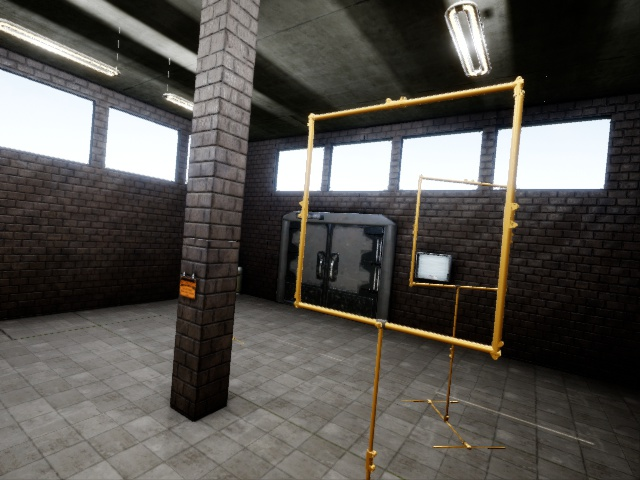
\includegraphics[width=\linewidth]{fig/daylight_1}
	\end{minipage}
	\begin{minipage}{0.4\linewidth}
	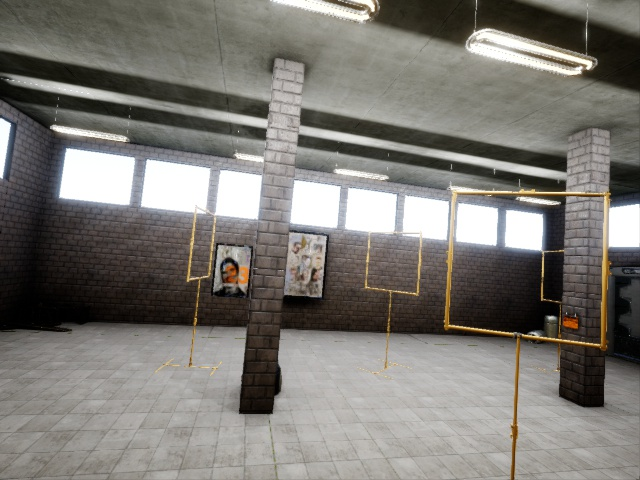
\includegraphics[width=\linewidth]{fig/daylight_2}
	\end{minipage}
\label{fig:daylight}
\caption{"Daylight" Room}
\end{figure}

\section{Model}

After our last experiment we hypothesized a much smaller model, learning are more shallow representation of the gate should be able to perform equally well if not better. \autoref{fig:architecture} shows the architecture of GateNet which is so far the yolo model with a smaller architecture. The class probabilities were removed from the loss function instead only 1 confidence value is predicted. The architecture was found in an iterative fashion. Starting from the blue part different configurations were tested until a decent performance could be achieved. As comparison the YoloV2 model has around 50 Mio. trainable parameters, TinyYolo around 15 Mio., GateNet only 1.5 Mio.

\begin{figure}
	\centering
	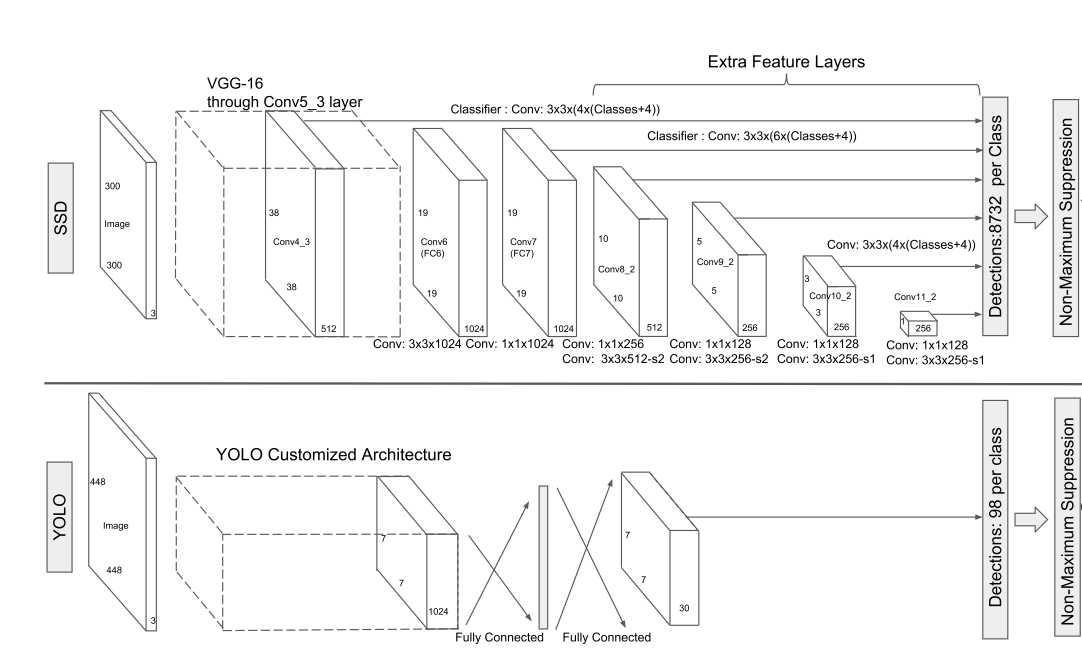
\includegraphics[width=0.9\linewidth]{fig/architecture}
	\label{fig:architecture}
	\caption{Architecture of GateNet, after each batch normalization leaky relu activation is applied}
\end{figure}

\section{Experiments}

We generate 3 training sets with 10 000 samples each. The distance as well as the angle towards a gate is limited, meaning there are no samples that contain gates that have an angle of less than 30 degrees towards the camera.
\begin{itemize}
	\item Basement. Contains images from the room of the previous report.
	\item Daylight. Contains only images from the room shown in \autoref{fig:daylight}.
	\item Mixed. Contains 5000 images from each of the datasets above. 
\end{itemize}

We generate 2 test sets with 500 samples for each room in the same way as the training data. Each model is trained on each training set and tested on each test set. Results can be seen in \autoref{fig:pr}.

\begin{figure}
	\centering
	\begin{minipage}{0.45\linewidth}
		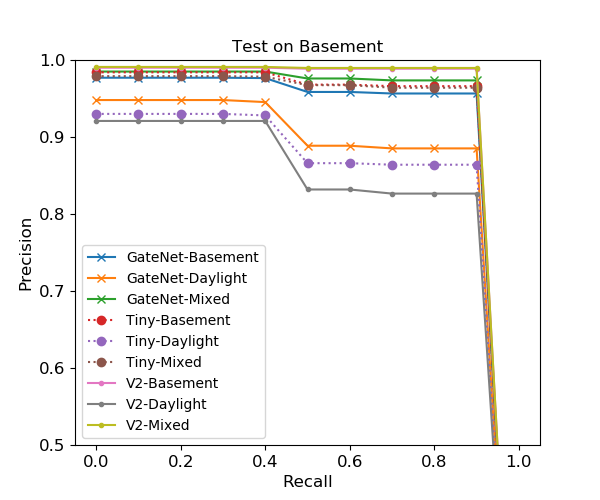
\includegraphics[width=\linewidth]{fig/pr_basement_all}
	\end{minipage}
	\begin{minipage}{0.45\linewidth}
		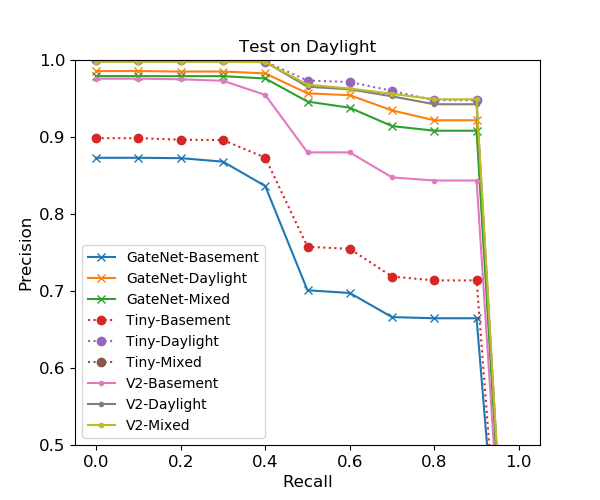
\includegraphics[width=\linewidth]{fig/pr_daylight_all}
	\end{minipage}
\end{figure}

First thing to notice is the huge improvement towards the last training. Limiting the training samples seem to have really benefited the model.

If we look at the performance of the models that have been trained in the basement room and tested in the daylight room we see quite a drop in performance. The most complex model yolov2 seem to have learned to most robust presentation as it looses only a bit of precision. The other way we see a smaller drop in performance for all models. It seems that the daylight set requires the model to learn a more robust representation, maybe because we have higher light contrasts due to the windows in the room. However, it could also be that the basement set has generally easier samples. Here the simplest model GateNet is the most robust one while v2 looses the most performance.

When comparing the performance of models that have been trained in both rooms to the models that have been trained in the same environment as tested, we see only small differences. The models are able to perform well in both environments. This is different to previous experiments where it seemed pretty hard to learn a general model. As we are interested in a robust general model we look closer at the performance of the models that have been trained on the mixed-dataset.


\begin{figure}
	\centering
	\begin{minipage}{0.30\linewidth}
		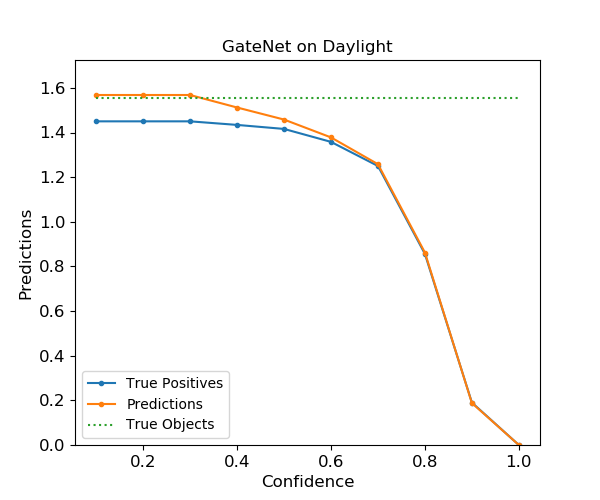
\includegraphics[width=\linewidth]{fig/detection_gate}
	\end{minipage}
	\begin{minipage}{0.30\linewidth}
		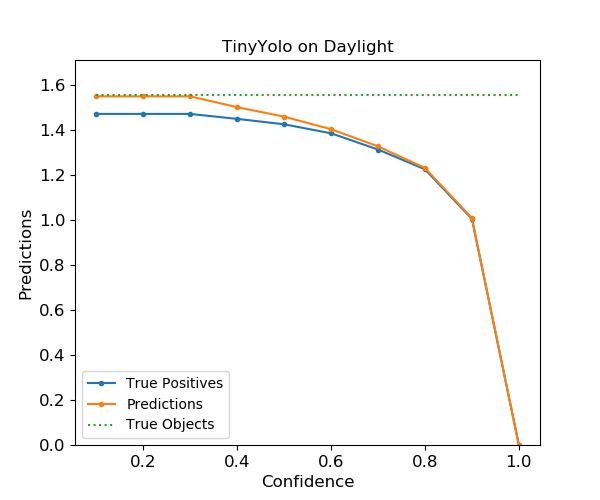
\includegraphics[width=\linewidth]{fig/detection_tiny}
	\end{minipage}
	\begin{minipage}{0.30\linewidth}
		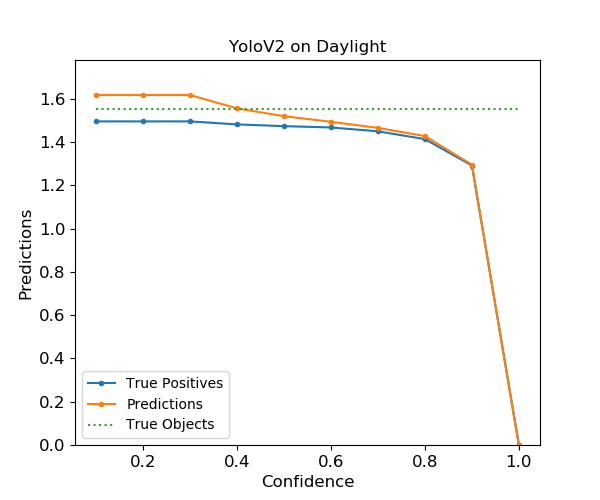
\includegraphics[width=\linewidth]{fig/detection_v2}
	\end{minipage}
\label{fig:conf}
\end{figure}

\autoref{fig:conf} shows the number of true positives/predictions over confidence. We see how the predictions resemble the number of objects in the image. Even at low confidence values the model does not produce a lot of false positives. At a confidence of 0.6 all models reach 100 \% precision, while differing in number of false negatives. While GateNet and TinyYolo have 0.2 false negatives, YoloV2 stays at 0.1 false negatives. It is also apparent how, as the model get more complex the model get more confident in their predictions.

Finally we can look at some predictions \autopageref{fig:examples}. We see GateNet on the left, YoloV2 on the right.

\begin{figure}
	\centering
	\begin{minipage}{0.3\linewidth}
		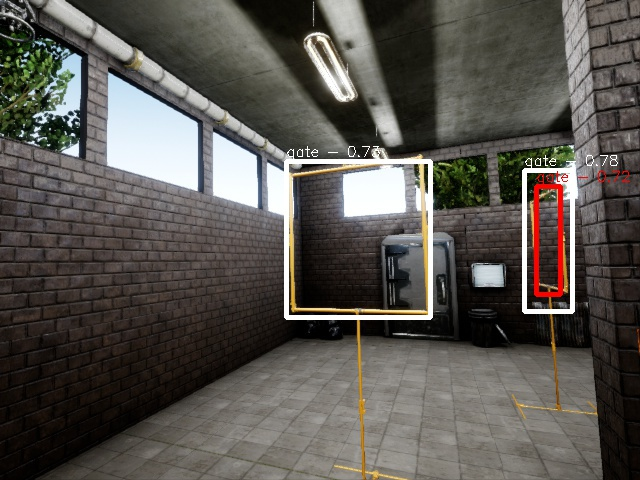
\includegraphics[width=\linewidth]{fig/gate_comp}
	\end{minipage}
	\begin{minipage}{0.3\linewidth}
		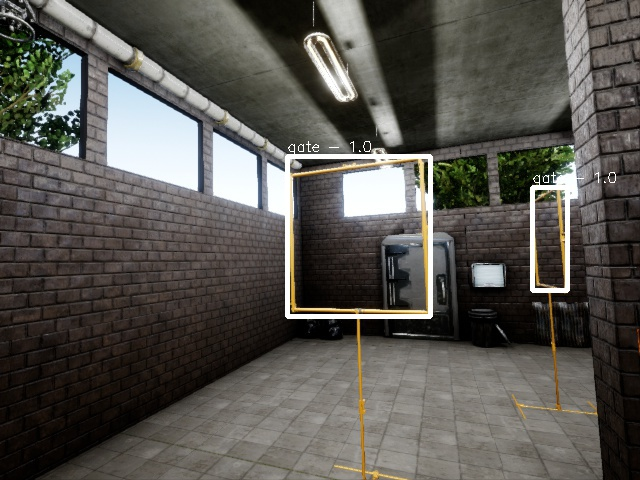
\includegraphics[width=\linewidth]{fig/v2_comp}
	\end{minipage}

	\begin{minipage}{0.3\linewidth}
	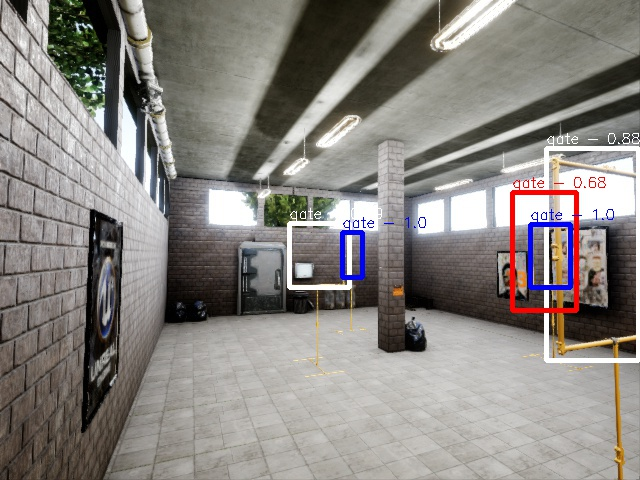
\includegraphics[width=\linewidth]{fig/gate_comp4}
	\end{minipage}
	\begin{minipage}{0.3\linewidth}
	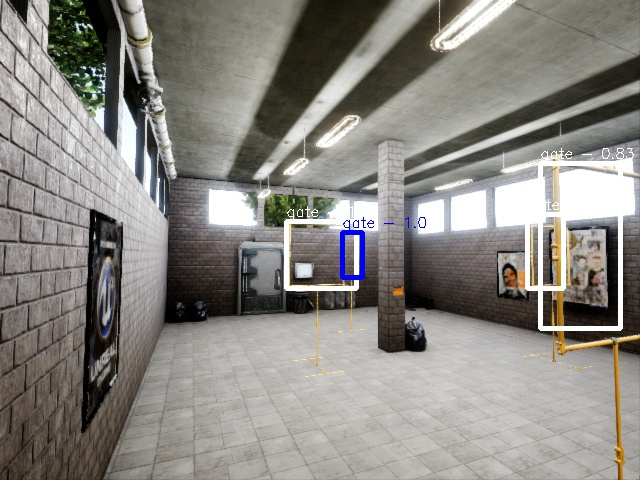
\includegraphics[width=\linewidth]{fig/v2_comp4}
	\end{minipage}
	\caption{GateNet tends to predict multiple boxes on the same gate or imprecise bounding boxes when gates are partially occluded or from a difficult angle.}

		\begin{minipage}{0.3\linewidth}
		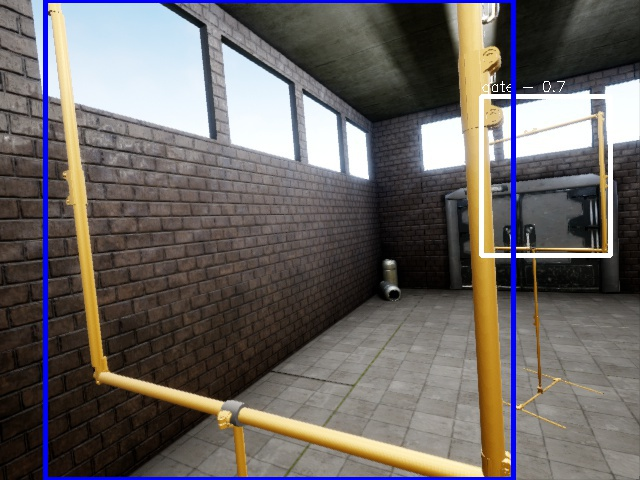
\includegraphics[width=\linewidth]{fig/gate_comp3}
	\end{minipage}
	\begin{minipage}{0.3\linewidth}
		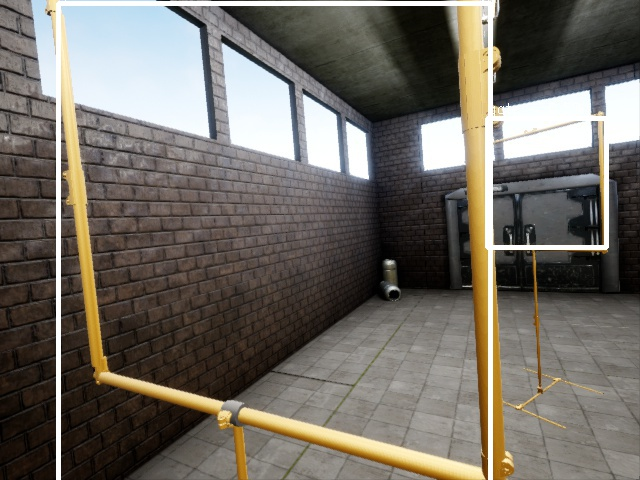
\includegraphics[width=\linewidth]{fig/v2_comp3}
	\end{minipage}
	\caption{GateNet can't handle occasions where the gate is very close to the camera. The reason might be due to the receptive field of the filters. As we reduced the depth of the network, the receptive field of the individual predictors also decreased.}
	
			\begin{minipage}{0.3\linewidth}
		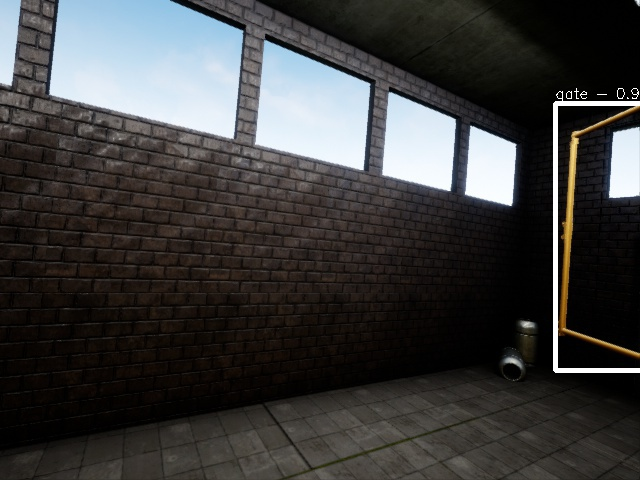
\includegraphics[width=\linewidth]{fig/gate_comp5}
	\end{minipage}
	\begin{minipage}{0.3\linewidth}
		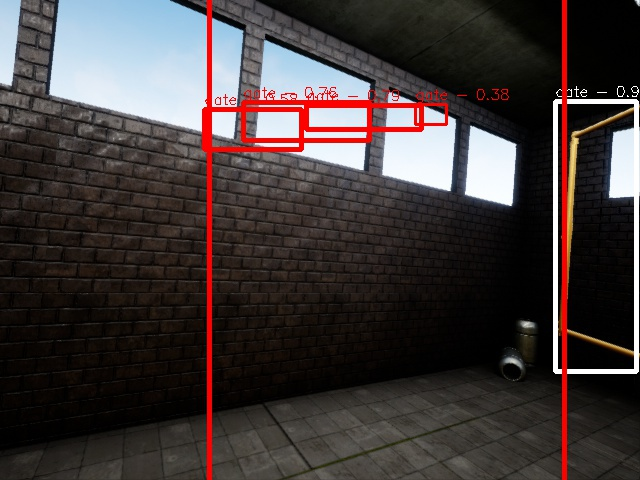
\includegraphics[width=\linewidth]{fig/v2_comp5}
	\end{minipage}
	\caption{YoloV5 seemed to have learned a weird pattern on this particular wall. There are several examples where it produces numerous bounding boxes like in this example. This did not happen to GateNet.}
		\label{fig:examples}
\end{figure}


\section{Conclusion}

\begin{itemize}
	\item The biggest problem was caused by high gate angles.
	\item With a much smaller model we can achieve almost similar performance in terms of precision and recall. Although this is very good, it does not confirm our assumption that the gate detection does not benefit from a deep representation. However, if we look at the images the reason for the better performance of YoloV2 might not be the deeper representation but rather the receptive field of the predictors.
\end{itemize}

\section{Next Step}
\begin{itemize}
	\item
\end{itemize}
%----------------------------------------------------------------------------------------


%----------------------------------------------------------------------------------------
%	BIBLIOGRAPHY
%----------------------------------------------------------------------------------------

\bibliographystyle{abbrv}

\bibliography{literature}

%----------------------------------------------------------------------------------------


\end{document}\grid
